Like in other web applications, in Shiny, you express server logic using reactive programming.
\\
The main idea of reactive programming is to specify the dependency graph so that when an input is changed, all related outputs are also updated. 
%for example, we don't need to tell an output to update because due to reactivity, the information is always updated. automatic, making the flow of an application considerably simpler.
\\
Reactivity is what makes applications responsive. Allows the application to update itself instantly whenever the user interacts with the application, requesting any visualization, with updated data.
\\
In Shiny, reactivity creates the illusion that changes to input values automatically flow to the outputs -- graphics, text, and tables that use the input --  and cause them to update. This flow behavior (such as current in a river or electricity) that pushes information from input to output is not real. In fact, in R an expression is only updated when it is executed (lazy evaluation).
\\
So, the idea is: the server re-execute the instructions very frequently, so it knows the input change very quickly, and acts as if it were bound to the input or as if input pushed its new value to the output.
\\
This is the approach that Shiny uses to create reactivity. This is why session R is busy when starting a Shiny application (for example, it is not possible to use the R console when the application is running). The server is using session R to monitor the application and rerun the expressions.
\\
However, Shiny takes this approach a step further, creating an alert system that lets you know exactly what expressions need to be rerun.
\\
Thus, although the server still checks the application at regular intervals (of microseconds), instead of rerunning each expression, it only executes the expressions that the alert system flagged as out of date. If alerts appear, the server executes all expressions that are out of date at the time - this event is called flush and is the key to reactivity as it allows the server to update the application as quickly as possible, appearing to flow instantly from inputs to outputs.
\\
We can see several examples of the use of reactivity in the code of our app. For example, in \verb!UI! (\ref{ui}) and in \verb!server! (\ref{server})
\begin{figure}[h]
\centering % para centralizarmos a figura
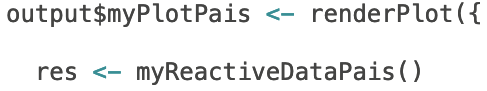
\includegraphics[width=0.6\textwidth]{images/reatividadeUI.png} 
\caption{reactivity:: UI}
\label{ui}
\end{figure}
\begin{figure}[h]
\centering % para centralizarmos a figura
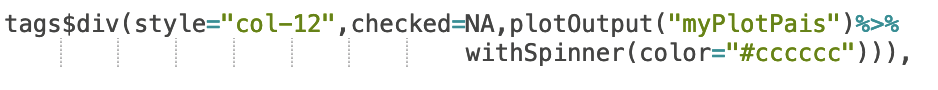
\includegraphics[width=\textwidth]{images/reatividadeSERVER.png} 
\caption{reactivity:: server}
\label{server}
\end{figure}
%In our app we use reactive functions, as it is a way to control which parts of the app are updated, avoiding unnecessary calculations that can slow down your app.

%In our application we use reactive functions as it is a way to control which parts of the application are updated, avoiding unnecessary calculations that can make your application slow.



%\begin{figure}[h]
%\centering % para centralizarmos a figura
%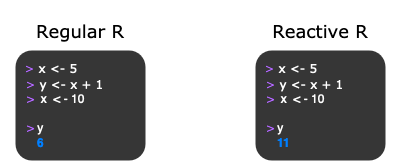
\includegraphics[width=7cm]{images/react.png} 

%\caption{Example of Regular R - Reactive R}
%\label{figura:qualquernome}
%\end{figure}




%For example, in our app //PUT AN EXAMPLE OF OUR APP
